\documentclass[11pt, a4paper, twocolumn]{article}
\usepackage[utf8]{inputenc}
\usepackage{url}
\usepackage{hyperref}
\usepackage[margin=1.5cm]{geometry}
\usepackage{graphicx}
\usepackage{amsmath}
\usepackage{amssymb}

%for code
\usepackage{listings}
\usepackage{color}

\definecolor{dkgreen}{rgb}{0,0.6,0}
\definecolor{gray}{rgb}{0.5,0.5,0.5}
\definecolor{mauve}{rgb}{0.58,0,0.82}

\lstset{frame=tb,
  language=Python,
  aboveskip=3mm,
  belowskip=3mm,
  showstringspaces=false,
  columns=flexible,
  basicstyle={\small\ttfamily},
  numbers=none,
  numberstyle=\tiny\color{gray},
  keywordstyle=\color{blue},
  commentstyle=\color{dkgreen},
  stringstyle=\color{mauve},
  breaklines=true,
  breakatwhitespace=true,
  tabsize=3
}

\usepackage{minted}

\title{
\begin{flushleft}

\includegraphics[width=3.5cm]{images/uibknew.eps}
\hfill

\includegraphics[width=1.8cm]{images/igslogo.png}
\hspace{0.3cm}

\includegraphics[width=0.9cm]{images/iislogo.png}
\end{flushleft}\vspace{0.5cm}
Visual Computing Project Report}
\author{Gerrit Mutschlechner \& Jonas Fauner \& Jonas Huber}

%-- more dense bibstyle
\let\oldthebibliography\thebibliography
\let\endoldthebibliography\endthebibliography
\renewenvironment{thebibliography}[1]{
  \begin{oldthebibliography}{#1}
    \setlength{\itemsep}{0em}
    \setlength{\parskip}{0em}
}
{
  \end{oldthebibliography}
}

\begin{document}


\maketitle

\thispagestyle{empty}


\section*{Introduction}
% Shortly describe the task of the project.
%Motivate and give the problem statement of the task.
%Add at least one reference (book \cite{Bridson08}, paper \cite{Zuenko20}, homepage \cite{lighthouse_timer}) via the 'sources.bib' and the 'cite' command.
%One final short paragraph about the own solution and the final results.

The main task of this project is to accurately detect facial features in images. This includes identifying faces, locating eyes within these faces smiles.
The problem encountered in your project arises from the inherent variability in the images, such as differences in lighting conditions, image quality, and distance from the camera. These factors significantly affect the system's ability to consistently and accurately identify facial features, specifically eyes and mouths. Additionally, the system struggles with face detection for individuals who are not facing the camera directly, such as those with their heads turned to the side. These challenges highlight the complexities involved in creating a robust facial feature detection system that can perform reliably across a diverse range of real-world scenarios. \cite{GreatLearning2023}
Our results were reasonably accurate, yet not flawless. We encountered issues where eye boxes were incorrectly placed where there were no heads. To mitigate this, we tried using a head box that only includes these eye boxes. Eyeglasses did not pose a problem, but numerous errors occurred with mouth detection, especially in areas where the image was overly dark or highly zoomed in. This highlights the challenges in achieving precise facial feature detection under varying image conditions.


\section*{Background}
%Shortly describe the necessary theory, e.g.~Blinn-Phong illumination model, fourier transformation, Gaussian blur.
%Show the employed theoretical formulas and/or more specialized math.
%\begin{align}
%    I_S = k_S M_S I_L \left( \cos \frac{\phi}{2} \right)^m = k_S M_S I_L \left( \mathbf{n} \cdot \mathbf{h} \right)^m
%\end{align}
 The key techniques include the use of Haar Cascade Classifiers, trained on numerous positive and negative images, to identify objects like faces, smiles, and eyes. The script enhances processing efficiency and accuracy through image resizing and grayscaling, standardizing dimensions and simplifying data. It utilizes the detectMultiScale function with adjustable parameters like scaleFactor and minNeighbors for precision in feature detection. The script's visual feedback mechanism involves drawing rectangles around detected features and displaying images for user interaction. These methods collectively enable effective detection and visualization of facial features in various images.

\section*{Method}
We used pretrained classifier from Github, for the smile and eyes detection \cite{OpencvDataHaarcascades}:
\begin{lstlisting}
faceCascade = cv2.CascadeClassifier('haarcascade_frontal face_default.xml')
eye_cascade = cv2.CascadeClassifier('haarcascade_eye.xml')
\end{lstlisting}

Iteratet over images
We resized the images
Used just Gray images
Used Face detection to lower false positives

used eye\_cascade.detectMultiScale(...)


\begin{lstlisting}
eyes = eye_cascade.detectMultiScale(roiGray, scaleFactor=1.1, minNeighbors=7, minSize=(20, 20)) 
smiles = smile_cascade.detectMultiScale(roiGray, scaleFactor=1.3 , minNeighbors=20 , minSize=(25, 25))

# Drawing rectangles around detected eyes and smiles
for (ex, ey, ew, eh) in eyes:
    cv2.rectangle(roiImg, (ex, ey), (ex+ew, ey+eh), (255, 0, 0), 2)
for (sx, sy, sw, sh) in smiles:
    cv2.rectangle(roiImg, (sx, sy), (sx+sw, sy+sh), (0, 255, 0), 2)
\end{lstlisting}
%
We found out, that ‚scaleFactor‘ and ‚minNeighbors‘ are important parameters used in the ‚detectMultiScale‘ method in OpenCV. These parameters are crucial for effectively detecting objects like faces, eyes, or smiles in images. \\\\
Following the purpose and impact of the parameters:\\\\
\textbf{scaleFactor}\\
The parameter specifies how much the image size is reduced at each image scale. This window is scaled down in size for each subsequent pass, allowing the algorithm to detect objects at various sizes (since an object can appear larger or smaller depending on its distance from the camera).
A smaller scaleFactor increases the chance of detecting smaller objects but also increases the computation time because more scales need to be processed. A larger scaleFactor reduces computation time but might miss smaller objects.
Typical Values are: 1.1, 1.2, 1.3 etc. 
A scale factor of 1.1 means that in each subsequent round, the search window is scaled down to 90\% of its previous size\\\\
\textbf{minNeighbors}\\
The minNeighbors parameter specifies the number of neighbors a rectangle should have to be retained as detection. After the size of the moving window is set by the scaleFactor, the algorithm needs to decide whether a given window location contains the object (like a face or an eye). minNeighbors sets the condition for reliability of detection.\\
A higher value results in fewer detections but with higher quality. A lower value increases the number of detections but also increases the number of false positives. \\
Typical Values are small integer values, like 3, 4, 5.\\\\
\textbf{minSize}\\
The minSize parameter sets the minimum size of the detection window. Any object smaller than this size will not be considered during the detection process.
In images where there is a lot of noise or smaller, irrelevant features, setting an appropriate minSize can help to reduce false positives.\\
Typical Values are [20, 20] or .\\\\
Especially we had to find the right balance for scaleFactor and minNeighbors:
\begin{itemize}
    \item If we are missing objects, we have to decrease scaleFactor or minNeighbors
    \item If we are getting to many false positives, we have to increase minNeighbors or scaleFactor
    \item Smaller scaleFactor uses more computational power, but that is not a problem for us, since we don’t use our application in real-time.
\end{itemize}
%


\section*{Results}

At the beginning we got poor results, after tuning these parameters the performance improved.

\begin{lstlisting}
faces = faceCascade.detectMultiScale(gray, scaleFactor=1.2 , minNeighbors=5, minSize=(30, 30))
for (x, y, w, h) in faces:
        # Extracting the region of interest (ROI) for the face in grayscale and color images
        roiGray = gray[y:y+h, x:x+w] 
        roiImg = img[y:y+h, x:x+w]

        # Drawing a rectangle around the detected face in the color image
        cv2.rectangle(img, (x, y), (x + w, y + h), (0, 0, 255), 2)

\end{lstlisting}




\begin{figure}[h]
 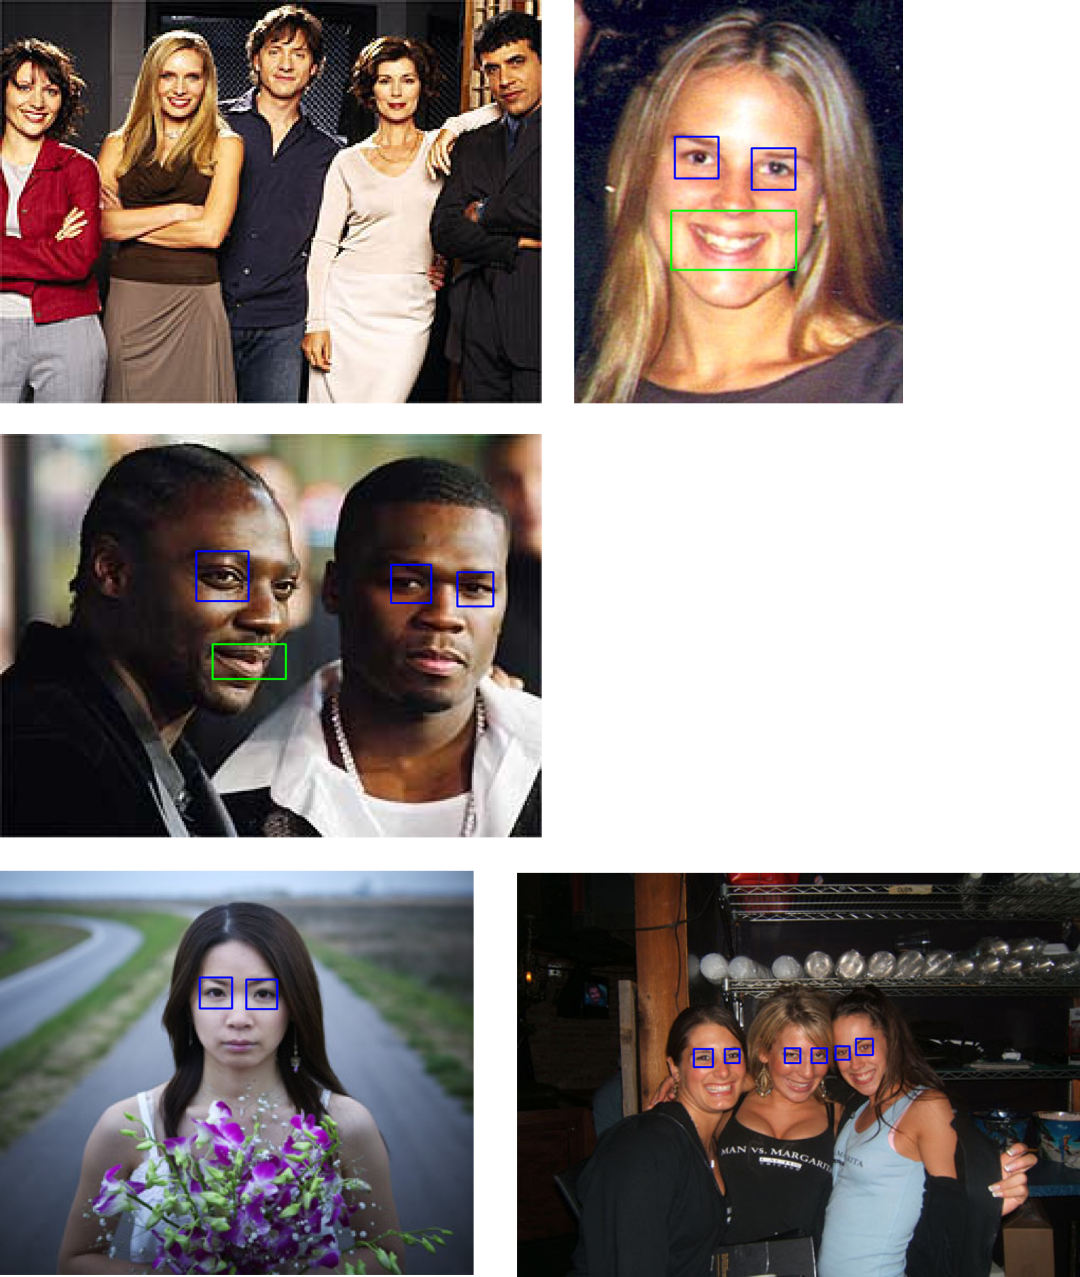
\includegraphics[width=1.0\columnwidth]{images/01_fewFalsePositives_fewDetected.png}
 \centering
 \caption{Few false positives but also a lot of smiles and eyes not detected.}
 \label{fig:01_fewFalsePositives}
\end{figure}

\begin{figure}[h]
 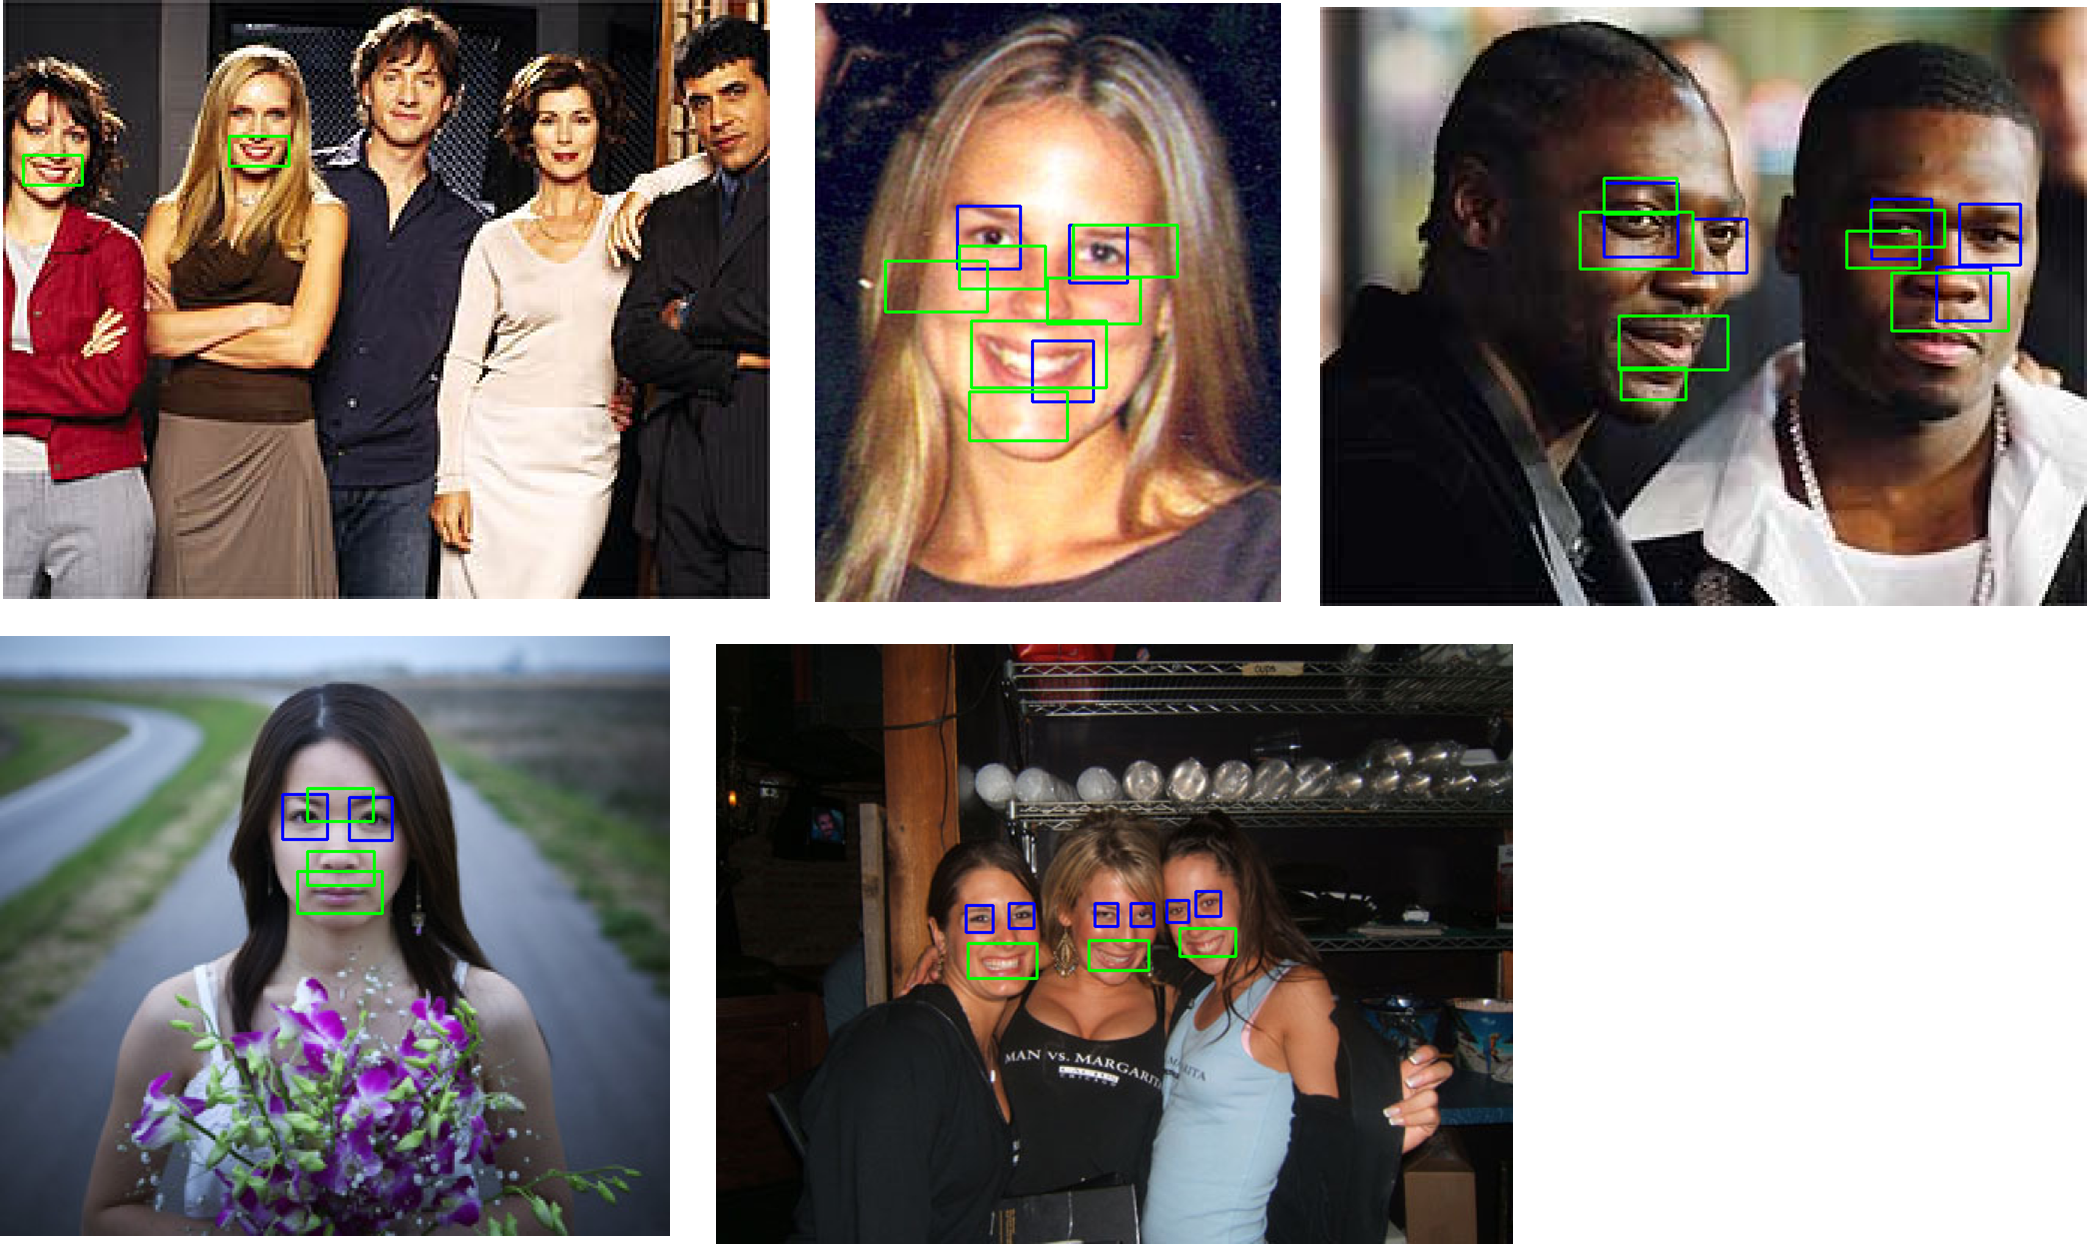
\includegraphics[width=1.0\columnwidth]{images/02_manyFalsePositives_manyDetected.png}
 \centering
 \caption{Many eyes and smiles detected, but also many false positives.}
 \label{fig:01_manyFalsePositives}
\end{figure}

\begin{figure}[h]
 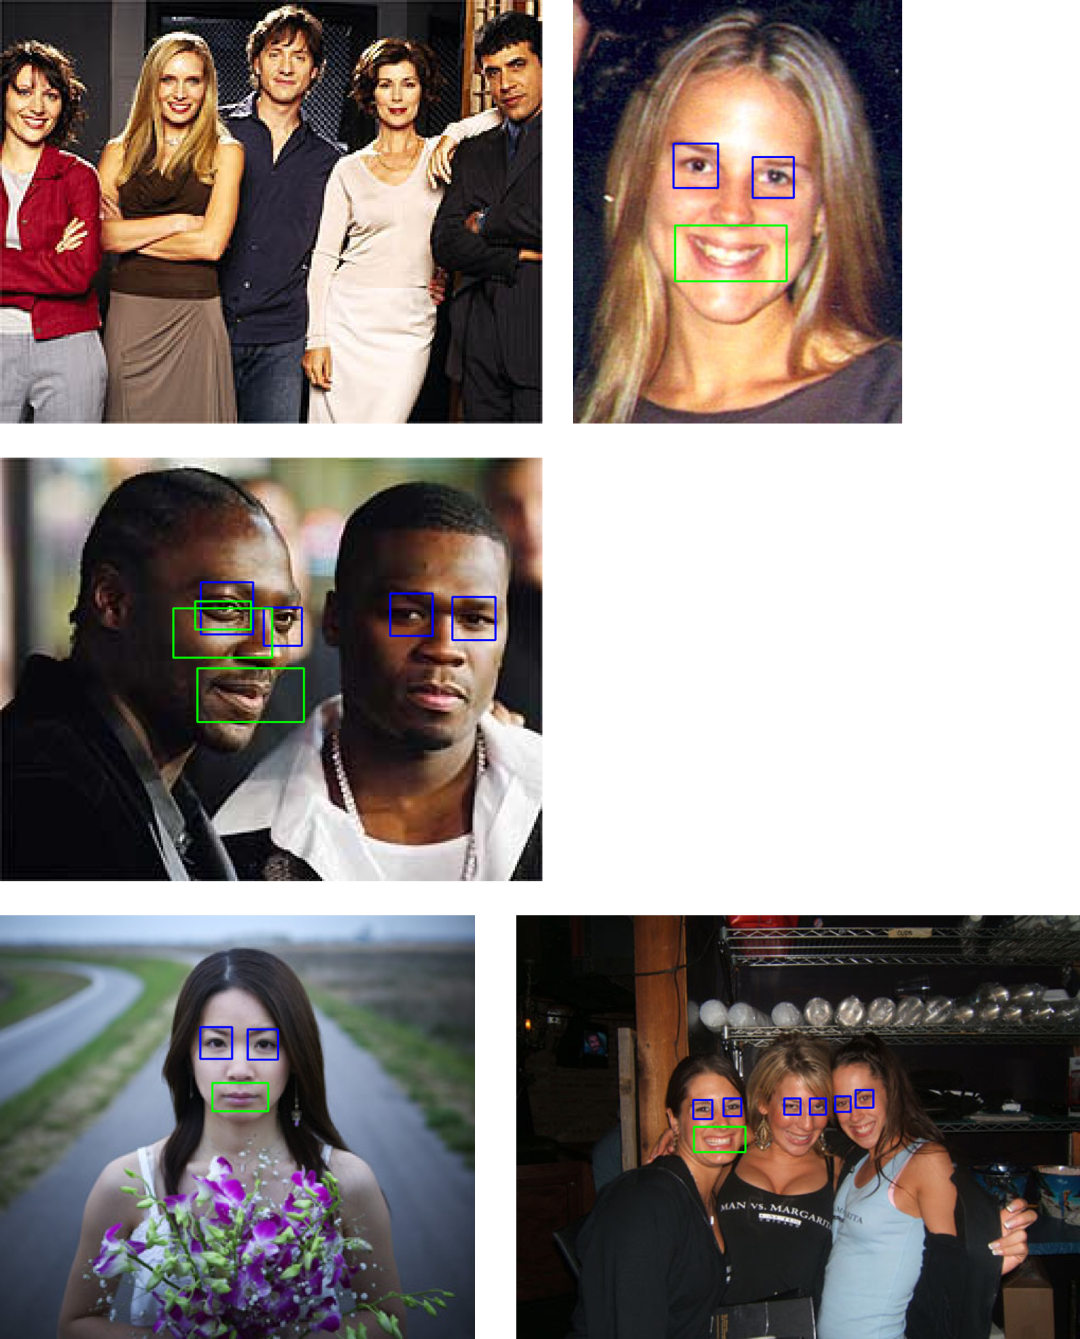
\includegraphics[width=1.0\columnwidth]{images/03_tradeof.png}
 \centering
 \caption{A tradeof between false positives and detected eyes and smiles.}
 \label{fig:03_tradeof}
\end{figure}

\begin{figure}[h]
 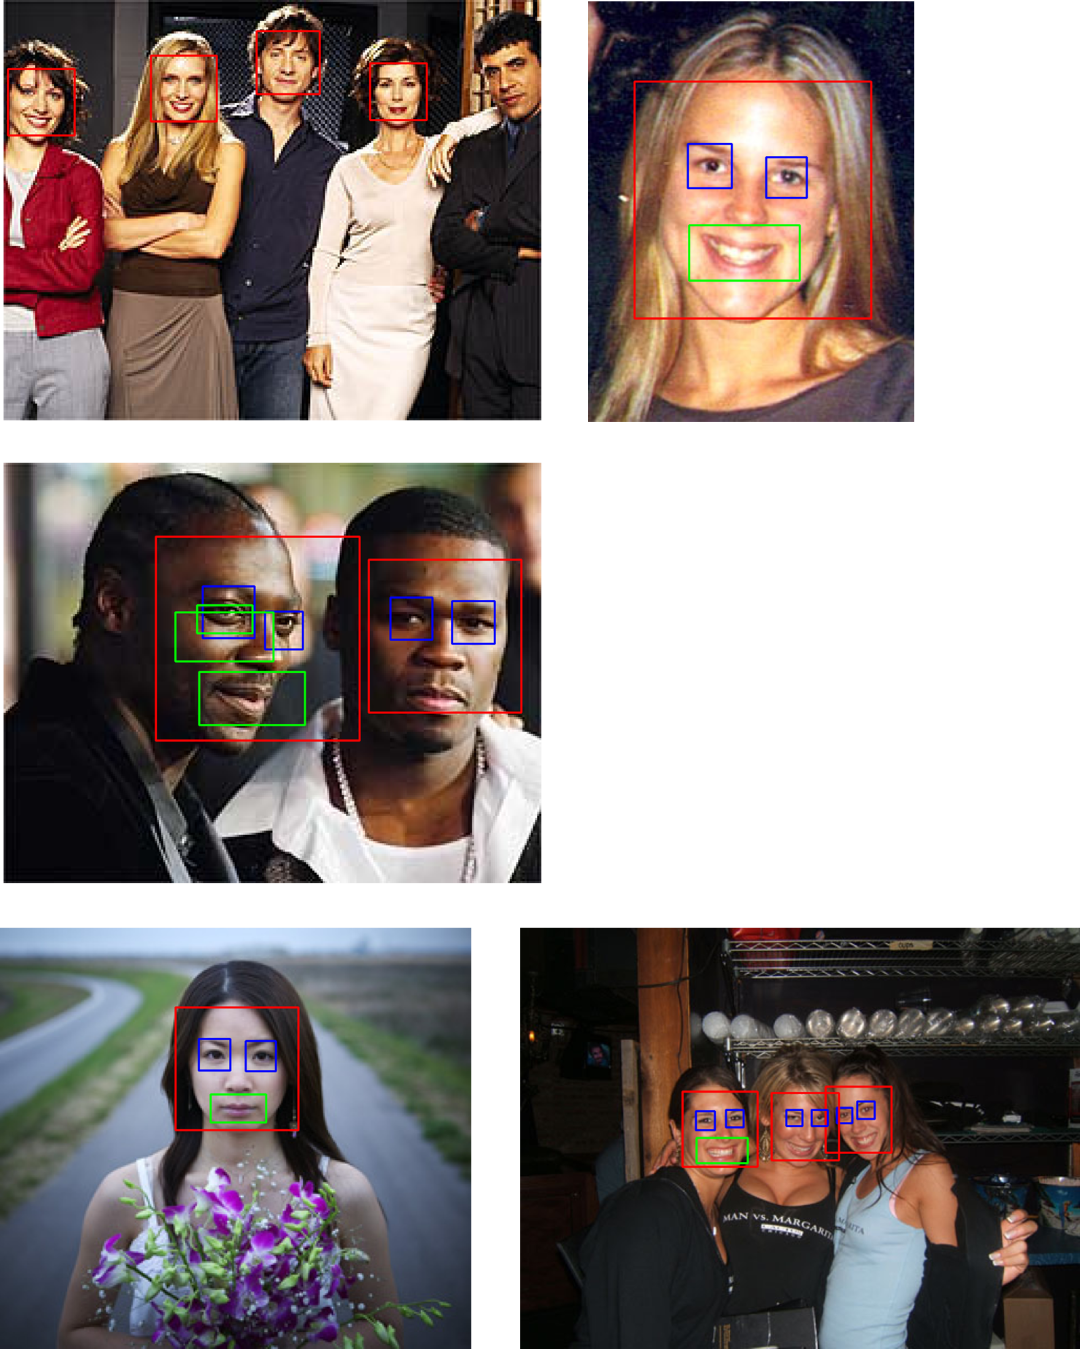
\includegraphics[width=1\columnwidth]{images/04_withFaceRectangle.png}
 \centering
 \caption{Face detection shown.}
 \label{fig:04_withFaces}
\end{figure}

%
\begin{figure}[h]
    \centering
    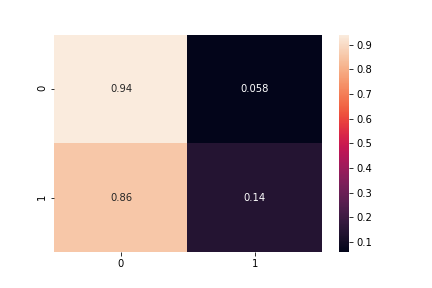
\includegraphics[width=0.4\textwidth]{images/confusion_matrix.png}
    \caption{Normalized Confusion Matrix}
    \label{fig:conf_matrix}
\end{figure}

\section*{Conclusion}


\bibliographystyle{plain}
\bibliography{sources}{}

%\bibliographystyle{ieeetr}



\end{document}
